\documentclass{article}

\usepackage{hyperref}
\usepackage{tikz}
\usepackage{rotating}

\usetikzlibrary{calc,positioning,shapes,shadows,arrows}

% tikz custom stuff
\tikzstyle{block} = [rectangle, draw, fill=blue!20, 
    text width=5em, text centered, rounded corners, minimum height=4em]
\tikzstyle{TextBox} = [rectangle, draw, fill=blue!20, 
    right, text width=4em, rounded corners]
\tikzstyle{line} = [draw, -latex']
\tikzstyle{cloud} = [draw, ellipse,fill=red!20, node distance=3cm,
    minimum height=2em]


\tikzstyle{startstop} = [rectangle, rounded corners,
    minimum width=3cm, minimum height=1cm,text centered,
    draw=black, fill=red!30]

\tikzstyle{decision} = [diamond, minimum width=3cm, 
    text width=5em, minimum height=1cm, text centered, draw=black, fill=green!30]


\tikzstyle{process} = [rectangle, minimum width=3cm,
    text width=20em, minimum height=1cm, text centered, draw=black, fill=orange!30]

\tikzstyle{arrow} = [thick,->,>=stealth]


\tikzset{
    hyperlink node/.style={
        alias=sourcenode,
        append after command={
            let     \p1 = (sourcenode.north west),
                \p2=(sourcenode.south east),
                \n1={\x2-\x1},
                \n2={\y1-\y2} in
            node [inner sep=0pt, outer sep=0pt,anchor=north west,at=(\p1)] {\hyperlink{#1}{\XeTeXLinkBox{\phantom{\rule{\n1}{\n2}}}}}
                    %xelatex needs \XeTeXLinkBox, won't create a link unless it
                    %finds text --- rules don't work without \XeTeXLinkBox.
                    %Still builds correctly with pdflatex and lualatex
        }
    }
}

\tikzset{square arrow/.style={to path={-- ++(0,.25) -| (\tikztotarget)}}}



\hypersetup{
    colorlinks=true, %set true if you want colored links
    linktoc=all,     %set to all if you want both sections and subsections linked
    linkcolor=black,  %choose some color if you want links to stand out
}

\title{Computer Science Coursework}
\date{}
\author{James Rand}

\def\tightlist{}

\newcommand{\placetextbox}[3]{% \placetextbox{<horizontal pos>}{<vertical pos>}{<stuff>}
    \setbox0=\hbox{#3}% Put <stuff> in a box
  \AddToShipoutPictureFG*{% Add <stuff> to current page foreground
      \put(\LenToUnit{#1\paperwidth},\LenToUnit{#2\paperheight}){\vtop{{\null}\makebox[0pt][c]{#3}}}%
  }%
}%

\makeatletter
\def\@seccntformat#1{%
    \expandafter\ifx\csname c@#1\endcsname\c@section\else
  \csname the#1\endcsname\quad
  \fi}
\makeatother

\begin{document}

\maketitle

\tableofcontents
\setcounter{tocdepth}{5}

\newpage

\section{Analysis}\label{analysis}

\subsection{Background}\label{background}

The main goal of this software to satisfy the client and their needs so
in order to do this successfully I need explain the situation my client
is in. My current client is a primary school teacher who would like to
use certain music during performances by the students. An example of a
song that would be needed by my client would a nursery rhyme like ``if
your happy and you know in clap your hands''. The current system in
place in virtually non existent by getting songs from online
and from CDs. It should be noted that the current method of playing this music
is through a CD player and that this application needs to be able to
burn the new music onto a CD so it can still be played through the CD
player.

Since the user is going to have little technical knowledge the program
needs to be easy to use which means I will need to have a GUI interface
instead of a CLI one. So far there is only demand by a single client but
I think that it should be able to have multiple users use it if need be.


\subsection{The problem}\label{the-problem}

Given this information the problem that I need to solve with this
application is to be able to get music from online and burn it to a disk
for my client to use. With this I can start to outline some objectives I
want this program to achieve.

\begin{itemize}
        \tightlist
    \item
        To be able to download music and store it
    \item
        Create playlists of these songs that my client can burn onto different
        disks
    \item
        Being able to burn these disks within the application
    \item
        Must be able to work on almost any environment without programs being
        pre-install 
\end{itemize}

For the first item on the list I need to consider where I get the music
from and whether it has copy right protection on it. My original thought
on this was to use YouTube as this by far has the most variety of music
on it and it would be familiar to people who use my application. The big
problem with this was copyright but after a little research I managed to
find that by editing the URL of the search you can search only for
copyright free videos which makes YouTube my preferred choice.

Next on the list I need to think how I would store this download music
into playlists. The most simple solution to this would be to use folders
where the folder name would be the name of the playlist and all of the
contents the song within the playlist. The problem with this is that it
would end up being slow and could take up considerable space as one song
could be in multiple playlists meaning that it would have to be copied
or use symlinks. Considering these factors it would be much more
efficient to use a database where all of the songs would be in a single
download folder where the database could organise them into different
playlists. This also means memory consumption would be at a minimum as I
could use ids to reference items in other table so there is little
repeated data. I also need to take into account that after a period of time
there could be a large number of songs meaning that I need to be able to store
them in a efficient manner.

Following the previous item we have to make sure that this application
will work on computers without being dependent on other programs. This
is critical for my client. The reasoning behind this is that this
application may be run upon a work computer where installing additional
programs is not feasible. Furthermore being able to transfer this
program using a USB and have it work on to. This also means I need to consider
network restrictions of when I run the program in school and how some websites
that I may use could be blocked.



\section{Design}\label{design}

This section will begin to explain how I plan to create this application.

\subsection{Outline}\label{outline}

The Qt library which is the library that I am using uses widgets which are window
like objects that can be embedded into one another to create a GUI. The bullets 
points below show how I plan to embed each of these widgets.

\begin{itemize}
    \item Main Window
        \begin{itemize}
            \item TabWidget
                \begin{itemize}
                    \item Download Tab
                        \begin{itemize}
                            \item search
                            \item preview
                        \end{itemize}
                    \item LibraryTab
                        \begin{itemize}
                            \item playlist list
                            \item tableview
                        \end{itemize}
                \end{itemize}
        \end{itemize}

\end{itemize}

The widget at the top of the hierarchy will be a child class of QMainWindow. This
allows me to use some of the functionality of QMainWindow like adding a menu bar
and shortcuts. I will then set the tabwidget as the central widget of this
allowing me to add tabs to my window. The next two bullet points Are the widgets
that the user will interact with to download and play music. The DownloadTab will
contain the an interface to preview the youtube video and then download it while
the LibraryTab will allow the user create playlists and organise the music. Figure 1
below illustrates this hierarchy graphically.

\begin{figure}
    \centering
    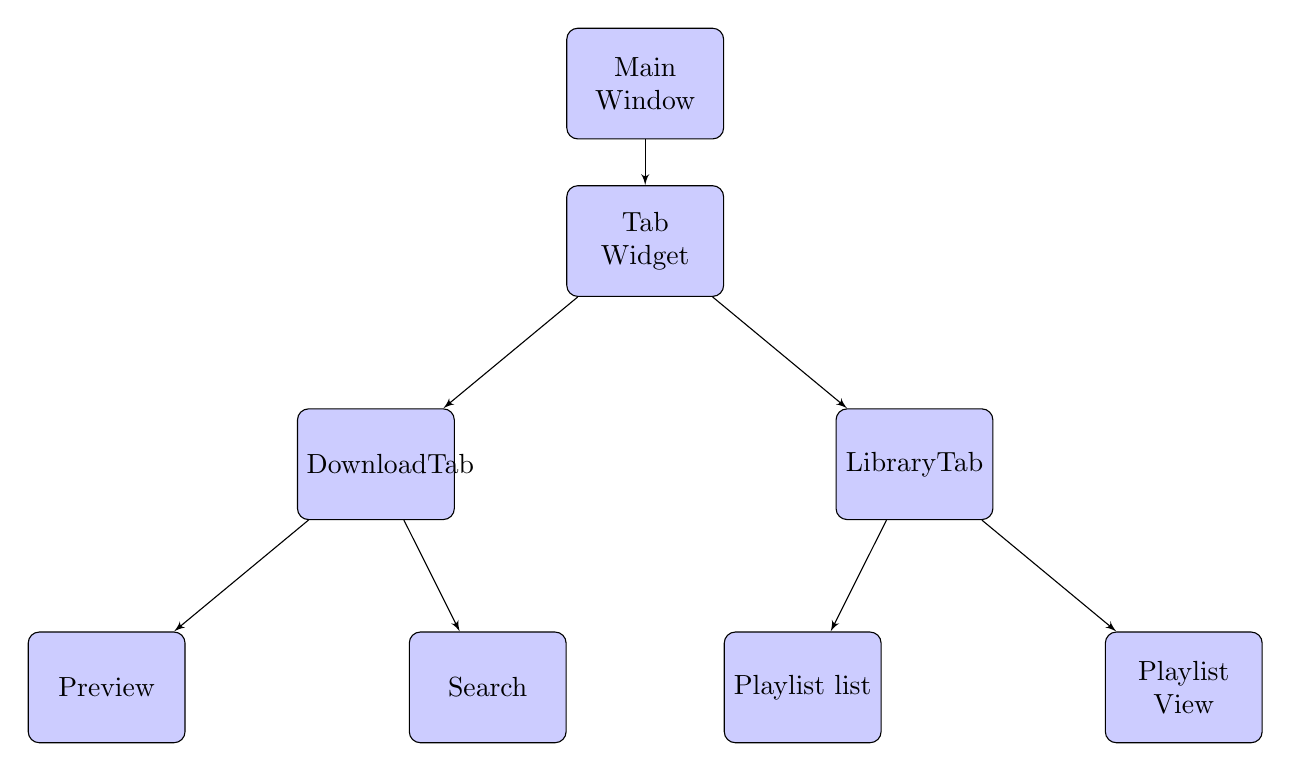
\begin{tikzpicture}[node distance = 2cm, auto]
        % Place nodes
        \node [block] (init) {Main Window};
        \node [block, below of=init] (TabWidget) {Tab Widget};
        \node [block, below left=of TabWidget] (DownloadTab) {DownloadTab};
        \node [block, below right=of TabWidget] (LibraryTab) {LibraryTab};
        \node [block, below left=of DownloadTab] (Preview) {Preview};
        \node [block, fill=none, draw=none, below right=of DownloadTab] (PlaceHolder) {};
        \node [block, left of=PlaceHolder] (Search) {Search};
        \node [block, right of=PlaceHolder] (PlaylistList) {Playlist list};
        \node [block, below right=of LibraryTab] (PlaylistView) {Playlist View};
        % Draw edges \path [line] (init) -- (identify);
        \path [line] (init) -- (TabWidget);
        \path [line] (TabWidget) -- (DownloadTab);
        \path [line] (TabWidget) -- (LibraryTab);
        \path [line] (DownloadTab) -- (Preview);
        \path [line] (DownloadTab) -- (Search);
        \path [line] (LibraryTab) -- (PlaylistList);
        \path [line] (LibraryTab) -- (PlaylistView);
    \end{tikzpicture}
    \caption{Layer Model} \label{fig:Layer Model}
\end{figure}

The two item on the graph above which has the most visual significance would be
DownloadTab and LibraryTab as they are the direct descendants of the Tab Widget.
Due to this fact I think that it is important to layout how I intend this two item to
look. The first that we will look at will be the Download Tab which is shown as Figure
~\ref{fig:DownloadTab Diagram}. There are quite a few objects on this diagram which are
not in the layer model (Fig ~\ref{fig:Layer Model}) these objects are to interact with
the two main widgets on the DownloadTab which are preview and searchlist. As the name
suggests the preview is to allow the user to view the video before downloading while.

Within GUI and network programming you often want one object to be notified when an event
happens to another. Fortunately Qt recognises this problem and has signals and slots to
solve it. To use these you need to use the emit to create a signal and the you can use 
a slot to listen out for that signal and run a procedure when that signal is received.
This is vital when interacting with the user as when the user clicks a button or interacts
with the interface a signal is emitted and I need to connect a slot up to these signals
to make the application work. 

With this knowledge I can start to explain how all of the classes come together and
function with the figures shown below. All of these figures are annotated and should
explain them in detail. It is important to know that the diagrams only show the
public procedures and functions currently. This is because I want to clearly line
out how they interact with one another. The only figure without this annotation is
figure ~\ref{fig:Struct layout} so I will explain it here. All of the structs that I
am describing occur in the classes VideoYoutube (Fig ~\ref{fig:VideoYoutube class layout})
and HttpHandler (Fig ~\ref{fig:HttpHandler class layout}) and the first to dive into is
download. This struct is to store information about the current downloaded video. The
first property "reply" is to store the response from the http request which will
especially important for checking for errors and making sure it has the right thing. The
next property "tempfile" is important for insurance reasons as the download may be
interrupted causing the file to be corrupt. In order to prevent this I thought it would
be best to create a temporary file that will be automatically deleted by the operating
system after a period of time. This means I can continually put data into this temporary
file and when the download file is finished save it into a permanent file. To have the
correct name to save the file to I have the title property. The "progress", 
"currentProgress" and "getProgress" are used to keep track of progress for the download
progress bar. The "segments" and "segmentPosition" is to allow the functionality to
download the video if it is cut into segments. "CurrentStatus" is to get the http status
code. Finally the "download()" procedure is to initiate the download process. 

The "fmtQuality" and "videoQuality" structs store the qualities and there relevant
urls. The first property of the "fmtQuality" struct is "quality" which stores the quality
that is listed by youtube. The "resolution", "video" and "audio" properties are to store
their qualities respectively. The procedure "fmtQuality" is the constructor to initialise 
all of these properties. The "videoQuality" has the same "quailty" property but also has
"audioUrl" and "videoUrl". These actually store the url to download the video. It should be 
noted that I put this property in "videoQuality" instead of "download" because there 
multiple urls for a video each different due to the quality. The "videoQuality" procedure
is different ways of initialising the properties and the operator is to compare the 
different qualities.

Finally the "jsMethod" struct is to store the the JavaScript code from youtubes code in
order to parse signatures to make the urls valid.

I need to also consider the data structure I am going to use for controlling the order of
the songs that will be played through LibraryTab. There are two data structures which
I am currently considering: Linkedlist and an array. A comparison table is shown in
Fig \ref{fig:Data structure table}. Based on the comparison and the ease of use it
belive that the easier and more efficient option would be to use an array.


%\break

\begin{figure}[h]
    \begin{center}
	\begin{tabular}{c | c}
	    LinkedList & Array \\ \hline
	    
    	\end{tabular}
    \end{center}
    \caption{Linkedlist vs array table} \label{fig:Data structure table}
\end{figure}


Another key design feature I need to implement is making the use of the program as
intuative as possible. Because of this I think the best way for the user to insert
songs and reorder them would be through a drag and drop system. This would require
me to set up various variables and features embbeded in qt which is described 
\href{http://doc.qt.io/qt-5/model-view-programming.html#using-drag-and-drop-with-item-views}
{here}.

\begin{figure}
    \centering
    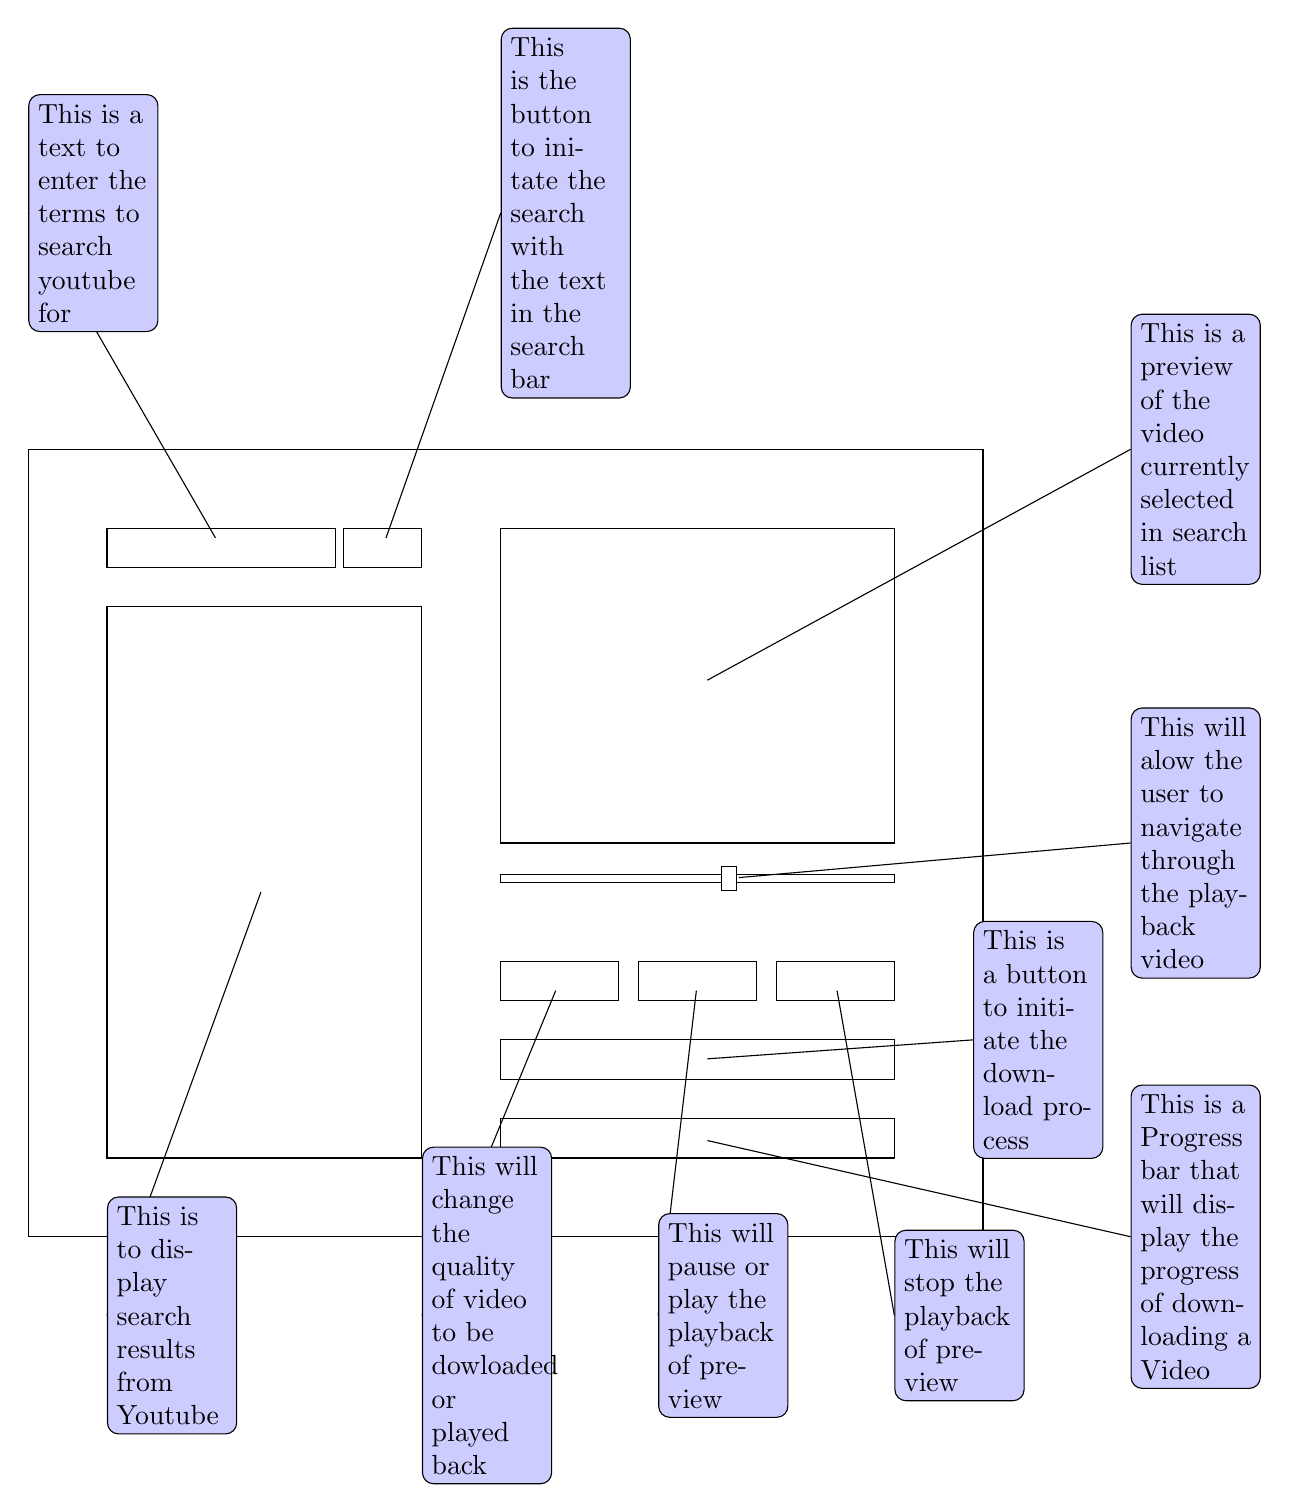
\begin{tikzpicture}[]
        \draw [fill=white] (0,0) rectangle (\textwidth,10) node[pos=0.5] (DownloadTab) {};
        \draw [] (3.9, 8.5) rectangle (1, 9) node[pos=0.5] (SearchBar) {}; %serch bar
        \draw [] (4, 8.5) rectangle (5, 9) node[pos=0.5] (SearchBtn) {}; %search btn
        \draw [] (1, 1) rectangle (5, 8) node[pos=0.5] (SearchList) {}; %search list
        \draw [] (11, 5) rectangle (6, 9) node[pos=0.5] (Preview) {}; %preview
        \draw [] (11, 4.5) rectangle (6, 4.6); %slider body
        \draw [fill=white] (9, 4.4) rectangle (8.8, 4.7) node[pos=0.5] (Slider) {}; %slider handle
        \draw [] (7.5, 3) rectangle (6, 3.5) node[pos=0.5] (QualitySelector) {}; %qualitySelector
        \draw [] (9.25, 3) rectangle (7.75, 3.5) node[pos=0.5] (PlayPauseBtn) {}; %play/pause
        \draw [] (11, 3) rectangle (9.5, 3.5) node[pos=0.5] (StopBtn) {}; %StopBtn
        \draw [] (11, 2) rectangle (6, 2.5) node[pos=0.5] (DownloadBtn) {}; %download btn
        \draw [] (11, 1.5) rectangle (6, 1) node[pos=.5] (ProgressBar) {}; %Progress Bar

        \draw (ProgressBar) -- (14, 0) node[TextBox, pos=1] {
            This is a Progress bar that will display the progress of downloading a Video
        };
        \draw (DownloadBtn) -- (12, 2.5) node[TextBox, pos=1] {
            This is a button to initiate the download process
        };
        \draw (StopBtn) -- (11, -1) node[TextBox, pos=1] {
            This will stop the playback of preview
        };
        \draw (PlayPauseBtn) -- (8, -1) node[TextBox, pos=1] {
            This will pause or play the playback of preview
        };
        \draw (QualitySelector) -- (5, -1) node[TextBox, pos=1] {
            This will change the quality of video to be dowloaded or played back
        };
        \draw (SearchList) -- (1, -1) node[TextBox, pos=1] {
            This is to display search results from Youtube
        };
        \draw (Slider) -- (14, 5) node[TextBox, pos=1] {
            This will alow the user to navigate through the playback video
        };
        \draw (Preview) -- (14, 10) node[TextBox, pos=1] {
            This is a preview of the video currently selected in search list
        };
        \draw (SearchBtn) -- (6, 13) node[TextBox, pos=1] {
            This is the button to initate the search with the text in the search bar
        };
        \draw (SearchBar) -- (0, 13) node[TextBox, pos=1] {
            This is a text to enter the terms to search youtube for
        };
    \end{tikzpicture}
    \caption{DownloadTab Diagram} \label{fig:DownloadTab Diagram}
\end{figure}


\begin{figure}
    \centering
    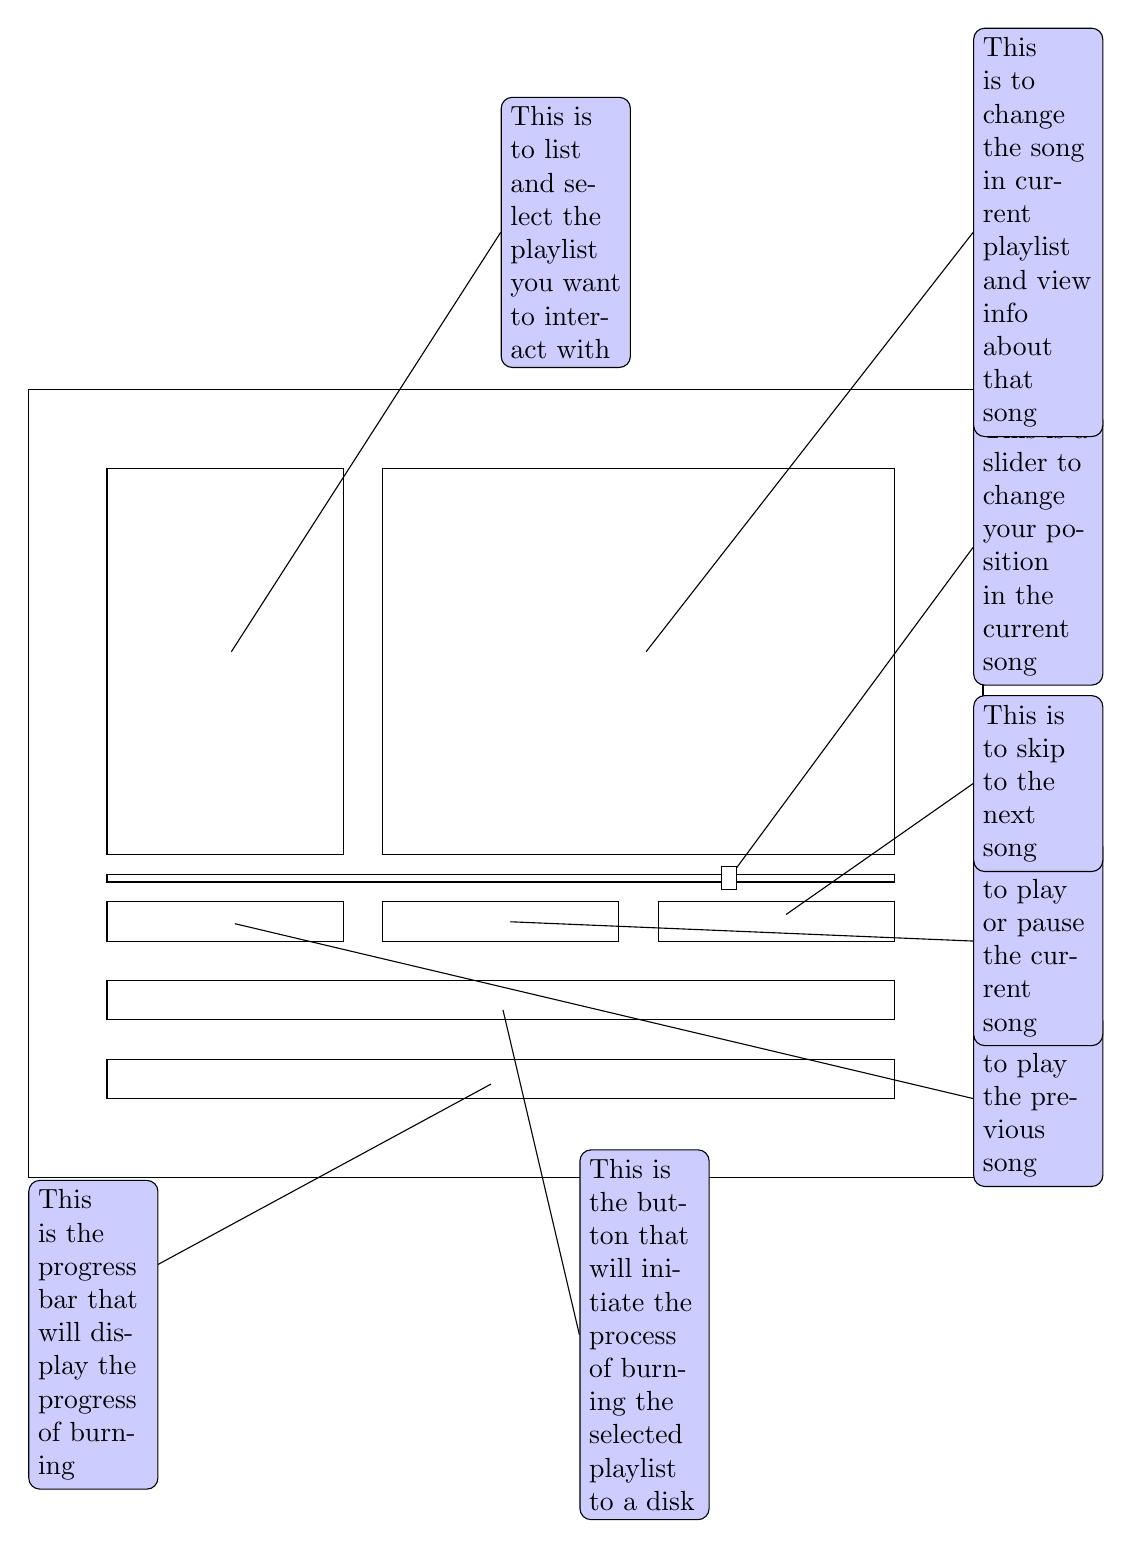
\begin{tikzpicture}[]
        \draw [] (0,0) rectangle (\textwidth, 10);
        \draw [] (1, 9) rectangle (4, 4.1) node[pos=0.5] (PlaylistListing) {}; %Playlist listing
        \draw [] (4.5, 9) rectangle (11, 4.1) node[pos=0.5] (SongSelector) {}; %Song selector
        \draw [] (11, 3.75) rectangle (1, 3.85); %slider body
        \draw [fill=white] (9, 3.65) rectangle (8.8, 3.95) node[pos=0.5] (Slider) {}; %slider handle    
        \draw [] (4, 3) rectangle (1, 3.5) node[pos=0.5] (Prev) {}; %prev Btn
        \draw [] (4.5, 3) rectangle (7.5, 3.5) node[pos=0.5] (PlayPause) {}; %play/pause
        \draw [] (11, 3) rectangle (8, 3.5) node[pos=0.5] (Next) {}; %next btn
        \draw [] (11, 2) rectangle (1, 2.5) node[pos=0.5] (BurnBtn) {}; %Burn btn        
        \draw [] (11, 1.5) rectangle (1, 1) node[pos=.5] (ProgressBar) {}; %Progress Bar         

        \draw (ProgressBar) -- (0, -2) node[TextBox, pos=1] {
            This is the progress bar that will display the progress of burning
        };
        \draw (BurnBtn) -- (7, -2) node[TextBox, pos=1] {
            This is the button that will initiate the process of burning the selected playlist to a disk
        };
        \draw (Prev) -- (12, 1) node[TextBox, pos=1] {
            This is to play the previous song
        };
        \draw (PlayPause) -- (12, 3) node[TextBox, pos=1] {
            This is to play or pause the current song
        }; 
        \draw (Next) -- (12, 5) node[TextBox, pos=1] {
            This is to skip to the next song
        };
        \draw (Slider) -- (12, 8) node[TextBox, pos=1] {
            This is a slider to change your position in the current song
        };
        \draw (SongSelector) -- (12, 12) node[TextBox, pos=1] {
            This is to change the song in current playlist and view info about that song
        };
        \draw (PlaylistListing) -- (6, 12) node[TextBox, pos=1] {
            This is to list and select the playlist you want to interact with
        };
    \end{tikzpicture}
    \caption{LibraryTab Diagram} \label{fig:LibraryTab Diagram} 
\end{figure}


\begin{figure}
    \centering
    \begin{tikzpicture}
        \begin{sideways}
            \node [] (tree) at (4, 4) {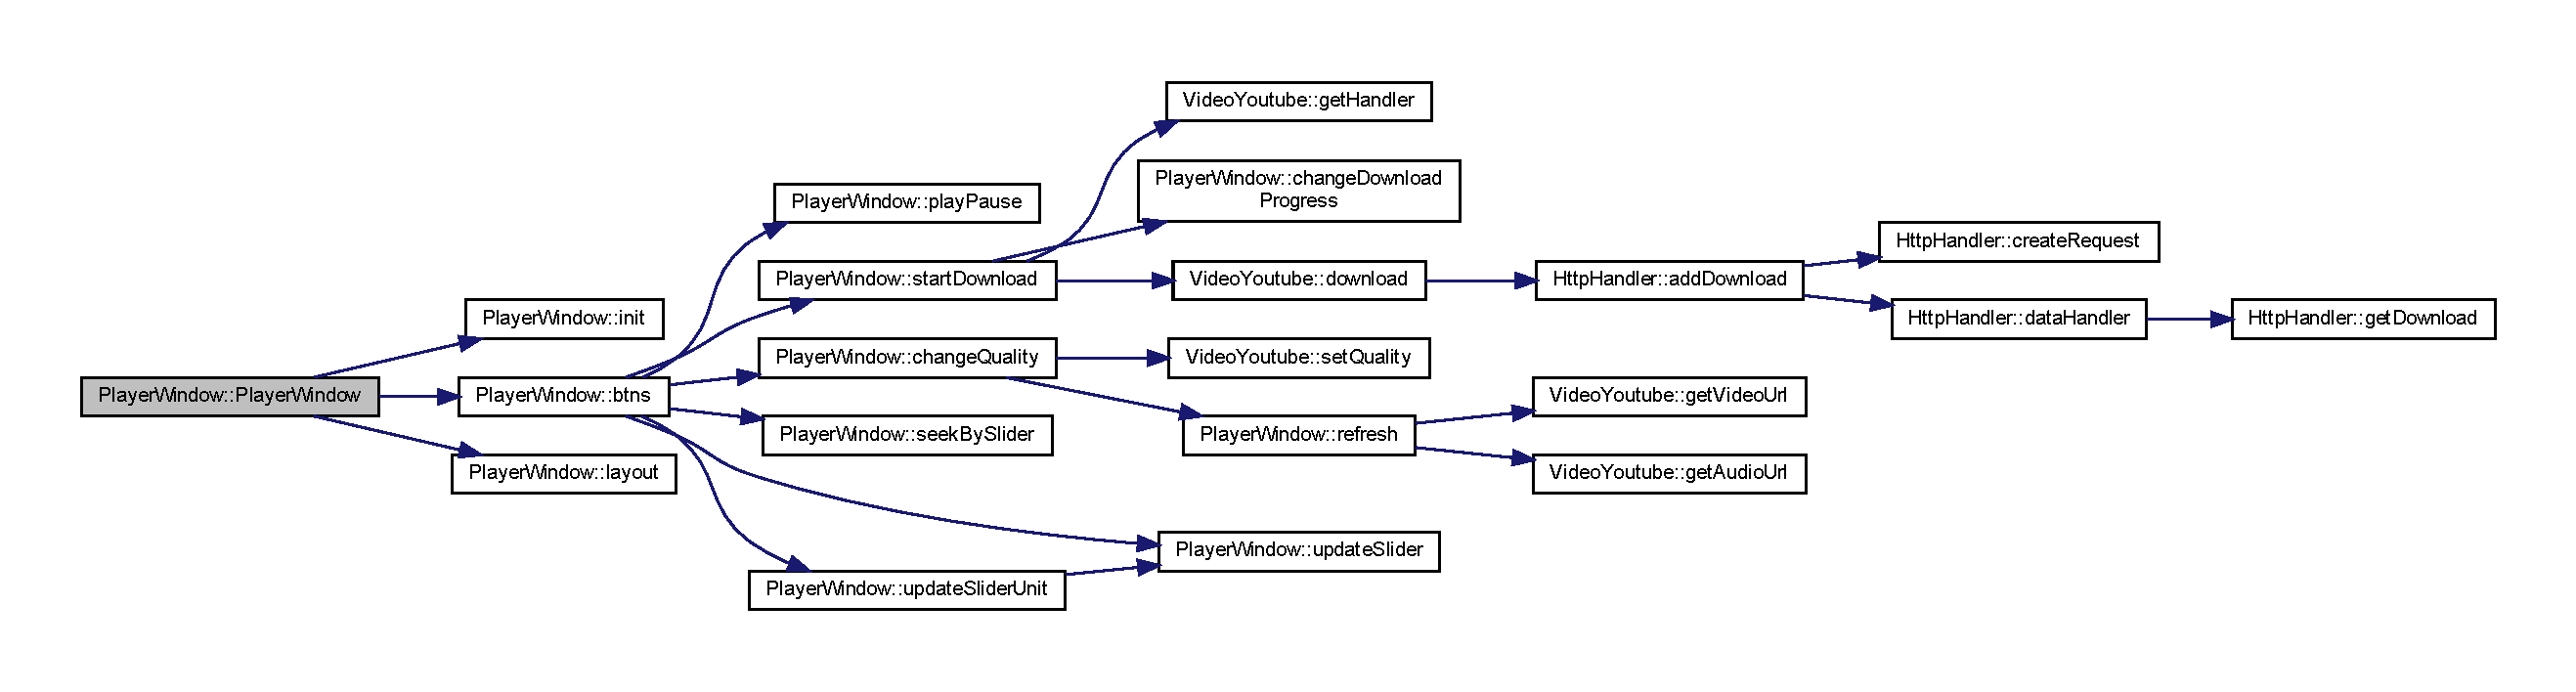
\includegraphics[width=\textheight]{classPdfs/classPlayerWindow_a88bd0544109c4b49dbba0adc29c16943_cgraph.pdf}};
        \end{sideways}
        \node [right of = tree] (inherit) {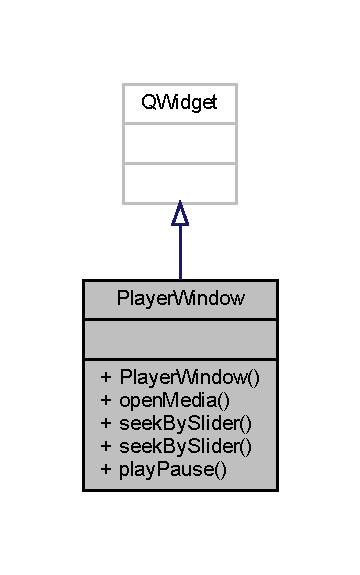
\includegraphics[]{classPdfs/classPlayerWindow.pdf}};
        \node [TextBox, above=0cm of inherit, text width = 30em] (textbox) {
            The class will be used to play media selected by the user and provide
            controls. This will be on both DownloadTab and LibraryTab meaning that
            the constructor will be called in both of these classes. The tree on the
            left describes what happens when you call the constructor. Since this is a
            class that will be visually displayed to the user this class inherits the
            QWidget. It also has the openMedia() procedure which is call by downloadtab
            to set the media after extracting the URL. Finally the seekBySlider and
            playPause are for the user to control the media.
        };
    \end{tikzpicture}
    \caption{PlayWindow class layout} \label{fig:PlayWindow class layout}
\end{figure}


\begin{figure}
    \centering
    \begin{tikzpicture}
        \begin{sideways}
            \node [] (tree) at (4, 4) {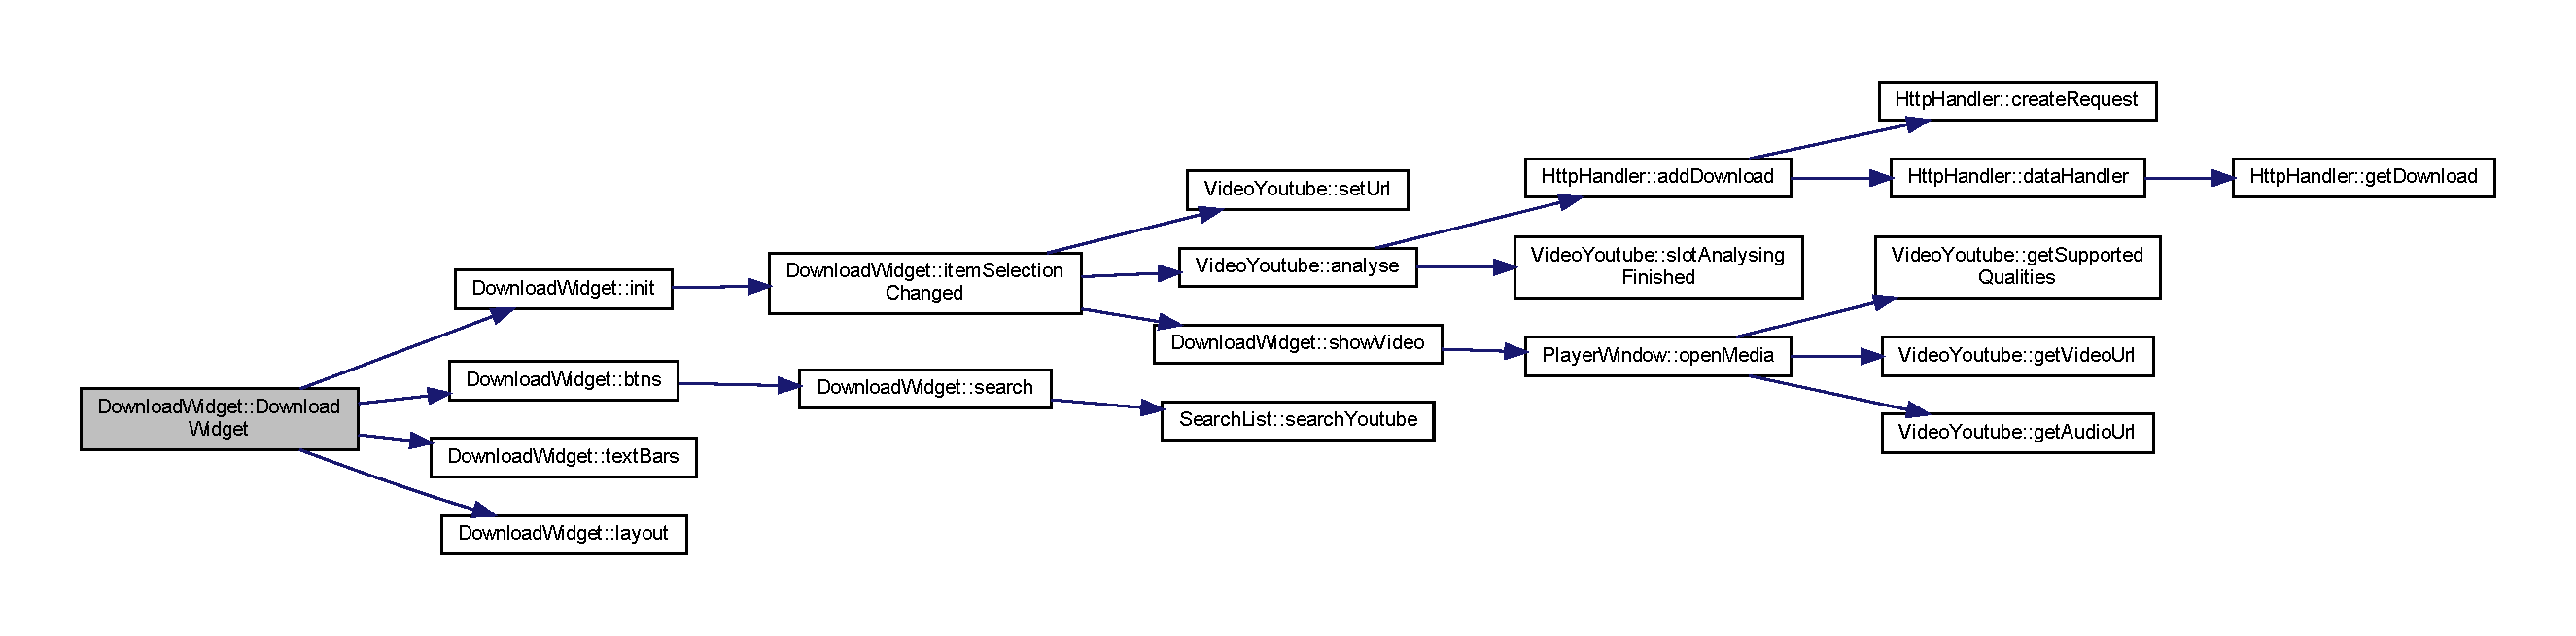
\includegraphics[width=\textheight]{classPdfs/classDownloadWidget_a623f84423fc0163ff5cd6b75000fffd5_cgraph.pdf}};
        \end{sideways}
        \node [right of = tree] (inherit) {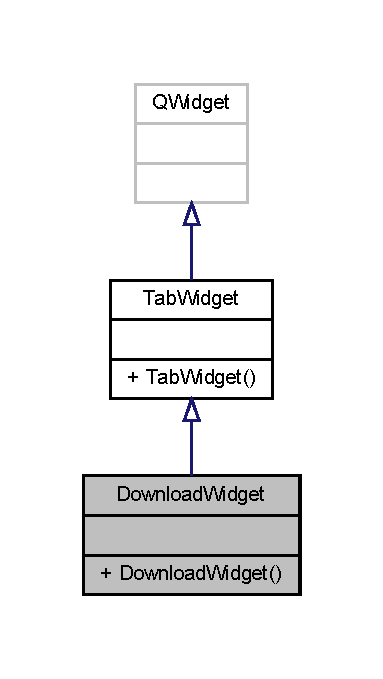
\includegraphics[]{classPdfs/classDownloadWidget.pdf}};
        \node [TextBox, above=0cm of inherit, text width = 30em] (textbox) {
        	The DownloadWidget class will be used to create the DownloadTab object. This
        	object will provide a canvas to put all of the features described in the
        	downloadTab diagram (Fig ~\ref{fig:DownloadTab Diagram}). It should be noted
        	this inherits from the TabWidget meaning it will be added as a tab 
        	automatically. The constructor will be called from the MainWindow. Finally
        	this class will act as a middle man for other classes like PlayerWindow
        	(Fig ~\ref{fig:PlayWindow class layout}).
        };
    \end{tikzpicture}
    \caption{DownloadWidget class layout} \label{fig:DownloadWidget class layout}
\end{figure}

\begin{figure}
    \centering
    \begin{tikzpicture}
        \begin{sideways}
            \node [] (tree) at (4, 4) {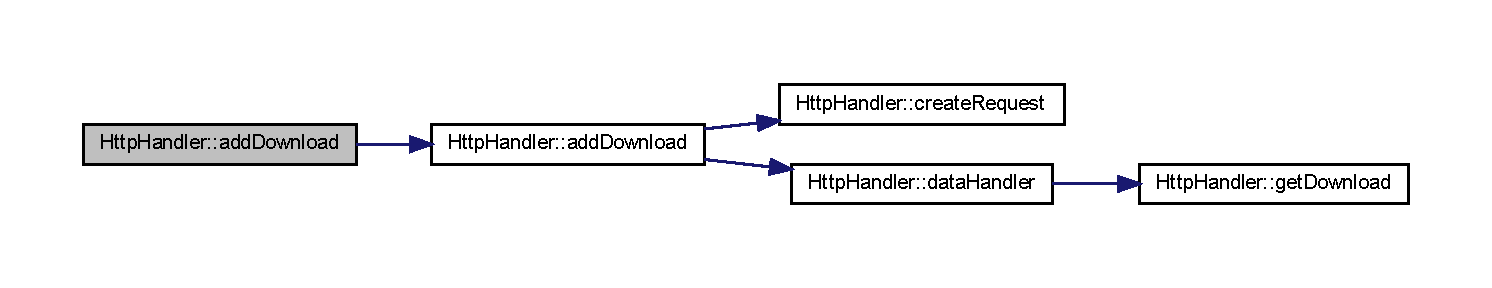
\includegraphics[width=\textheight]{classPdfs/classHttpHandler_ade64572cb953620fd483bc669c1e9178_cgraph.pdf}};
        \end{sideways}
        
        \node [right of = tree] (inherit) {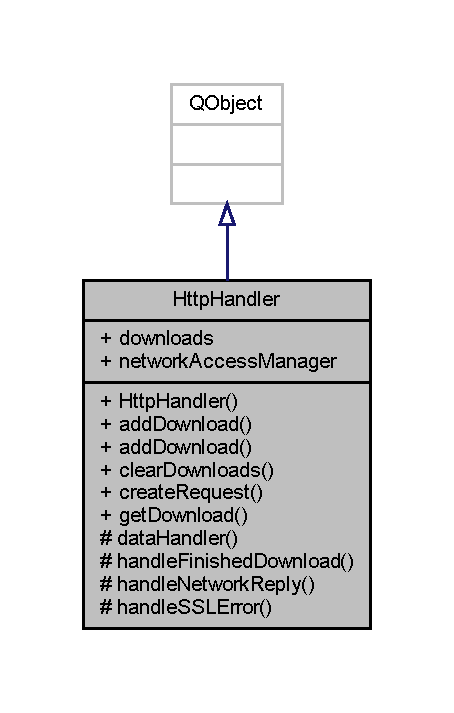
\includegraphics[]{classPdfs/classHttpHandler.pdf}};
        \node [TextBox, above=0cm of inherit, text width = 30em] (textbox) {
        	For this class the first thing that you know is that it inherits from QObject
        	instead of QWidget or a derivative of QWidget. This means that this class
        	has no visual representation but completely backend. The point of this class
        	is to perform all of the networking required. I decided to put all of it
        	into a seperate class because many errors can occur with network requests
        	so proper error handling is a must. Due to the fact that you often have to
        	wait for network requests to finished this class has numerous slots like
        	dataHandler to process the the finshed download. The final two things that
        	should be noted is the data members downloads and networkAcessManager.
        	The member downloads is a QList of the download struct, see (Fig ). The
        	networkAcessManager is a QNetworkManager which is Qt class that allows
        	you to make network requests.
        };
    \end{tikzpicture}
    \caption{HttpHandler class layout} \label{fig:HttpHandler class layout}
\end{figure}

\begin{figure}
    \centering
    \begin{tikzpicture}
        \begin{sideways}
            \node [] (tree) at (4, 4) {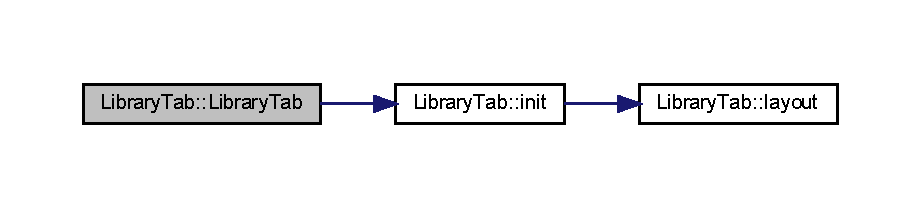
\includegraphics[width=\textheight]{classPdfs/classLibraryTab_a928c981ca174c41d75e5296d4623d5a2_cgraph.pdf}};
        \end{sideways}
        
        \node [right of = tree] (inherit) {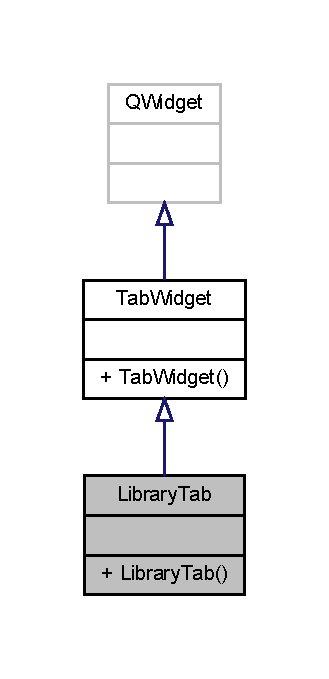
\includegraphics[]{classPdfs/classLibraryTab.pdf}};
        \node [TextBox, above=0cm of inherit, text width = 30em] (textbox) {
        	Similarly to DownloadWidget this is a child of TabWidget meaning it is one
        	of the two tabs and provides a canvas to put widgets on. Fig
        	\ref{fig:LibraryTab Diagram} shows how inten it to look. This class
        	will be the middle man for all of the data handling. Within the 
        	constructor all of the objects shown in Fig \ref{fig:LibraryTab Diagram}
        	will be initialized and then layed out in the layout procedure.
        };
    \end{tikzpicture}
    \caption{LibraryTab class layout} \label{fig:LibraryTab class layout}
\end{figure}

\begin{figure}
    \centering
    \begin{tikzpicture}
        \begin{sideways}
            \node [] (tree) at (4, 4) {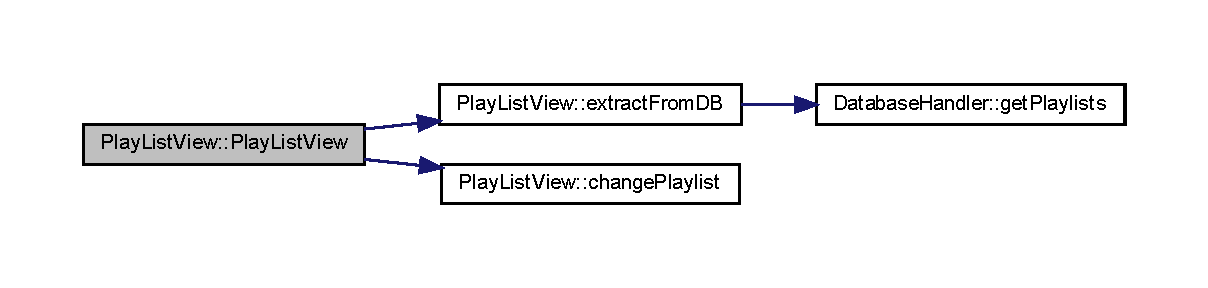
\includegraphics[width=\textheight]{classPdfs/classPlayListView_ac84c4c57fc29e6b775c2bc8bc5fed55e_cgraph.pdf}};
        \end{sideways}
        
        \node [right of = tree] (inherit) {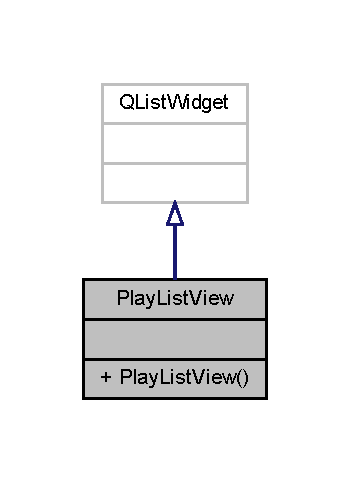
\includegraphics[]{classPdfs/classPlayListView.pdf}};
        \node [TextBox, above=0cm of inherit, text width = 30em] (textbox) {
			This class is called by LibraryWidget and is used to list the playlists
			that the user has and allow the user to place songs and edit the playlists.
			It should be noted that instead of a standard QWidget being used a QListWidget
			is used. This still has a visual representation but instead of being a blank
			canvas it lists items that you can add with the addItem procudure.
        };
    \end{tikzpicture}
    \caption{PlaylistView class layout} \label{fig:PlaylistView class layout}
\end{figure}

\begin{figure}
    \centering
    \begin{tikzpicture}
        \node [right of = tree] (inherit) {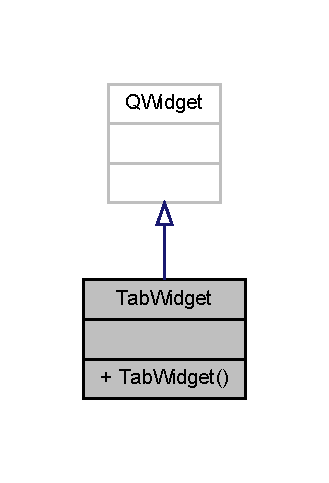
\includegraphics[]{classPdfs/classTabWidget.pdf}};
        \node [TextBox, above=0cm of inherit, text width = 30em] (textbox) {
			Unlike the other class this class is abstract. This means that it should
			always be a parent class in use and never called directly. The reasoning
			behind this is that I want a way that I could add classes automatically.
			This would also mean that if in the future I want to style my tabs I can
			easily do so by applying styles to this which would apply to the children.
        };
    \end{tikzpicture}
    \caption{TabWidget class layout} \label{fig:TabWidget class layout}
\end{figure}

\begin{figure}
    \centering
    \begin{tikzpicture}
        \begin{sideways}
            \node [] (tree) at (4, 4) {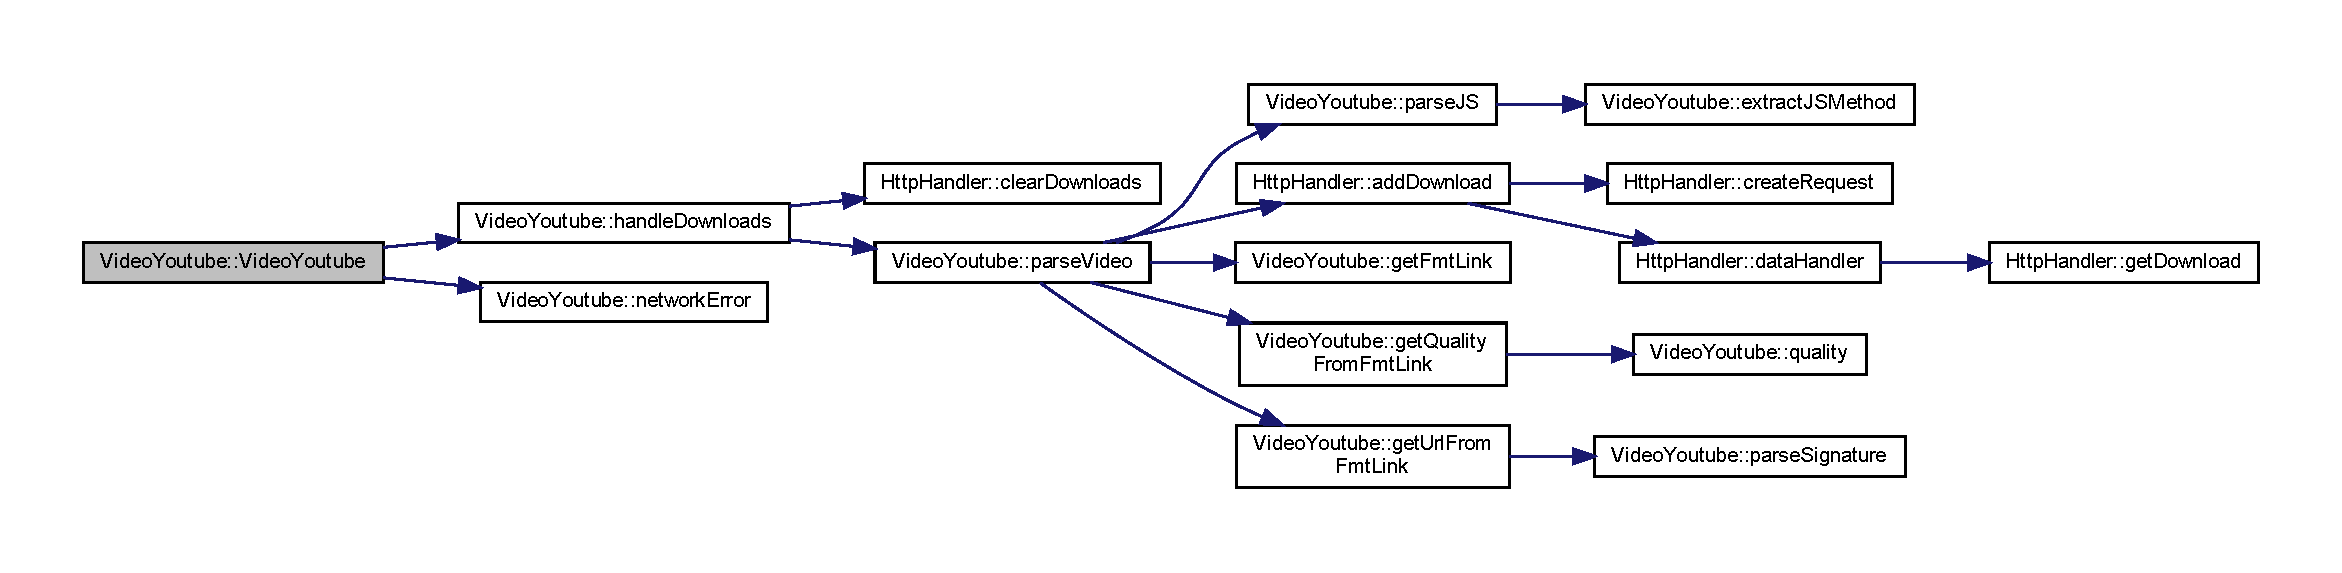
\includegraphics[width=\textheight]{classPdfs/classVideoYoutube_a80afcc31ca007b32108976d2158be9ce_cgraph.pdf}};
        \end{sideways}
        
        \node [right of = tree] (inherit) {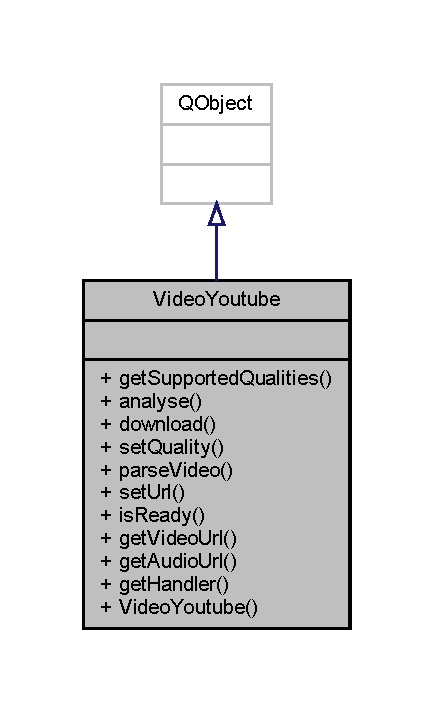
\includegraphics[]{classPdfs/classVideoYoutube.pdf}};
        \node [TextBox, above=0cm of inherit, text width = 30em] (textbox) {
			This class is used to represent the currently selected video from the
			search on the download tab. The main objective of this class is with the
			use of HttpHandler (Fig \ref{fig:HttpHandler class layout}) to extract the
			url of the actual youtube video which is done in the parseVideo procedure.
			Once the url has been retrived the getVideoUrl and the getAudioUrl functions
			provide objects like preview the url to play the video. The download procedure
			will pass the audio url onto the HttpHandler so that it can be downloaded
			and added to the database. Finally to repeat the process you need to set
			a new webpage url with setUrl and call the analyse procedure.
        };
    \end{tikzpicture}
    \caption{VideoYoutube class layout} \label{fig:VideoYoutube class layout}
\end{figure}

\begin{figure}
    \centering
    \begin{tikzpicture}
        \begin{sideways}
            \node [] (tree) at (4, 4) {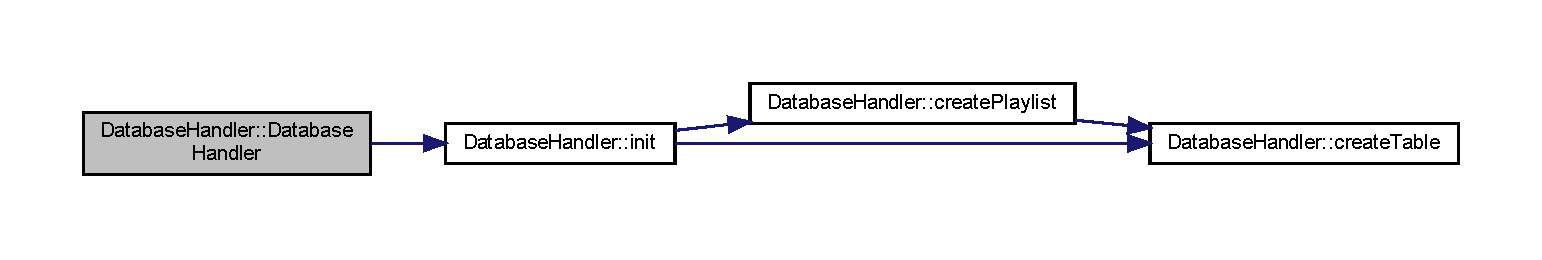
\includegraphics[width=\textheight]{classPdfs/classDatabaseHandler_a6f3d7ae8a73f534059dc5667b29eb0d2_cgraph.pdf}};
        \end{sideways}
        
        \node [right of = tree] (inherit) {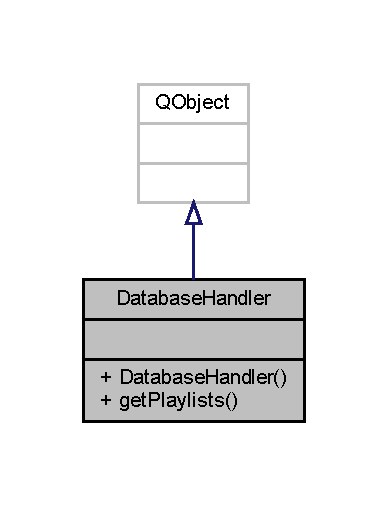
\includegraphics[]{classPdfs/classDatabaseHandler.pdf}};
        \node [TextBox, above=0cm of inherit, text width = 30em] (textbox) {
			This class is meant to handle all of the database function and is called
			by the LibraryWidget class. The should create all of the tables needed to
			represent the tables and organise everything. Like the HttpHandler class
			this class is a child of QObject showing that it is completely backend
			and has no visual representation.
        };
    \end{tikzpicture}
    \caption{DatabaseHandler class layout} \label{fig:DatabaseHandler class layout}
\end{figure}

\begin{figure}
    \begin{tikzpicture}[node distance=\textwidth /3]
        \node [] (download) {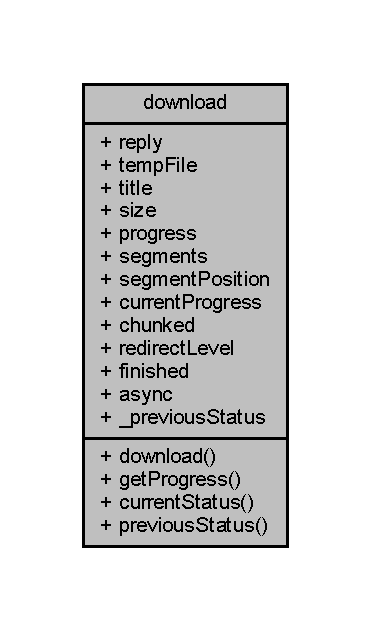
\includegraphics{classPdfs/structdownload}};
        \node [right of=download] (fmtQuality) {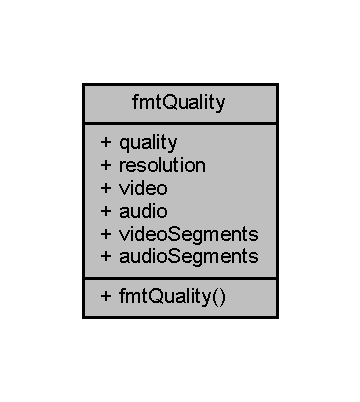
\includegraphics{classPdfs/structfmtQuality}};
        \node [below=0.0mm of  download.south] (videoQuality) {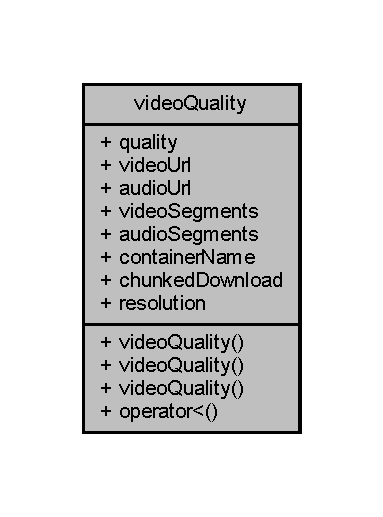
\includegraphics{classPdfs/structvideoQuality}};
        \node [right of=videoQuality] (jsMethod) {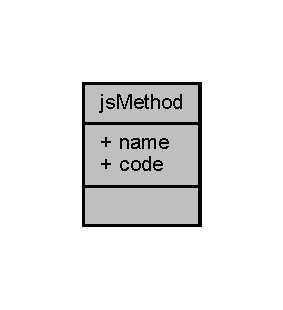
\includegraphics{classPdfs/structjsMethod}};
    \end{tikzpicture}
    \caption{Struct layout} \label{fig:Struct layout}
\end{figure}

\break
\subsection{DatabaseHandling}\label{DatabaseHandling}

As mention previously I decided that I would use a database to keep track of the
downloaded music. To do this I will have one main table that will have any
downloaded song automatically inserted into it. This table will be called "AllSongs"
. This "AllSongs" table with contain 5 columns which I will describe here.
The first column is the "id" columns which will be use to order the data
and to refrence the data inside "AllSongs". Because of this id will be an
integear with each one being unique and auto increment. The second column
is "TrackName" which as the title suggest will be a text field containing
the name of the download song. The next two columns will be "artists" and
"genre" which will both be integears to reference values in the artist and
genere tables. This will avoid duplicates. These tables will have an id field
identical to the AllSongs table and the artist and genere columns will
reference values using this field. Finally there will be the duration
file which is a double that will hold the length of the song in mineuts.

To further avoid duplications any playlist created by the user will refrence
the songs in "AllSongs".In order to allow these refrences I will need to use join
statements in sql. I need to use this statement as I still want the artist and 
genere columns in the users playlist without having to create this additional columns.
By using select with these join statement along with the where clause I should
be able to grab all data that has the same id.

A requirement by my client is the ability to reorder the songs. My approach
to this is to switch the id of the two songs to switch them in the view.
Due to both id's having the uniqure property I will need to use the id as
0 for a temp value. This should be relatively simple with sql update statements

Another database quirk that I need to take into consideration is when the user
deletes a song in the playlist as this will cause there to be gaps in the
ids of tables. This is probolmatic as I cannot get the right id by getting 
the rowid. There are two ways I could solve this: I update all of the ids
greater that the deleted item so there are no gaps or allow gaps and find
a way of selecting a row of data in the database by how far down it is.
The first option is a bad idea as this means changing id which are going
to be used as relations and it may become time consuming for large
amount of rows. The second option is much better but I was original unsoure
of how to acheive it untill I discovered the "OFFSET" clause. With this
I can offset a select statement n rows down the table making this task
trivial.

\subsection{NetworkHandling}\label{NetworkHandling}

As remarked previously a key part to this project is the process
of extracting the video url from youtube so it can be previewed
and the sound be downloaded. This section describes this process.



\begin{figure}
    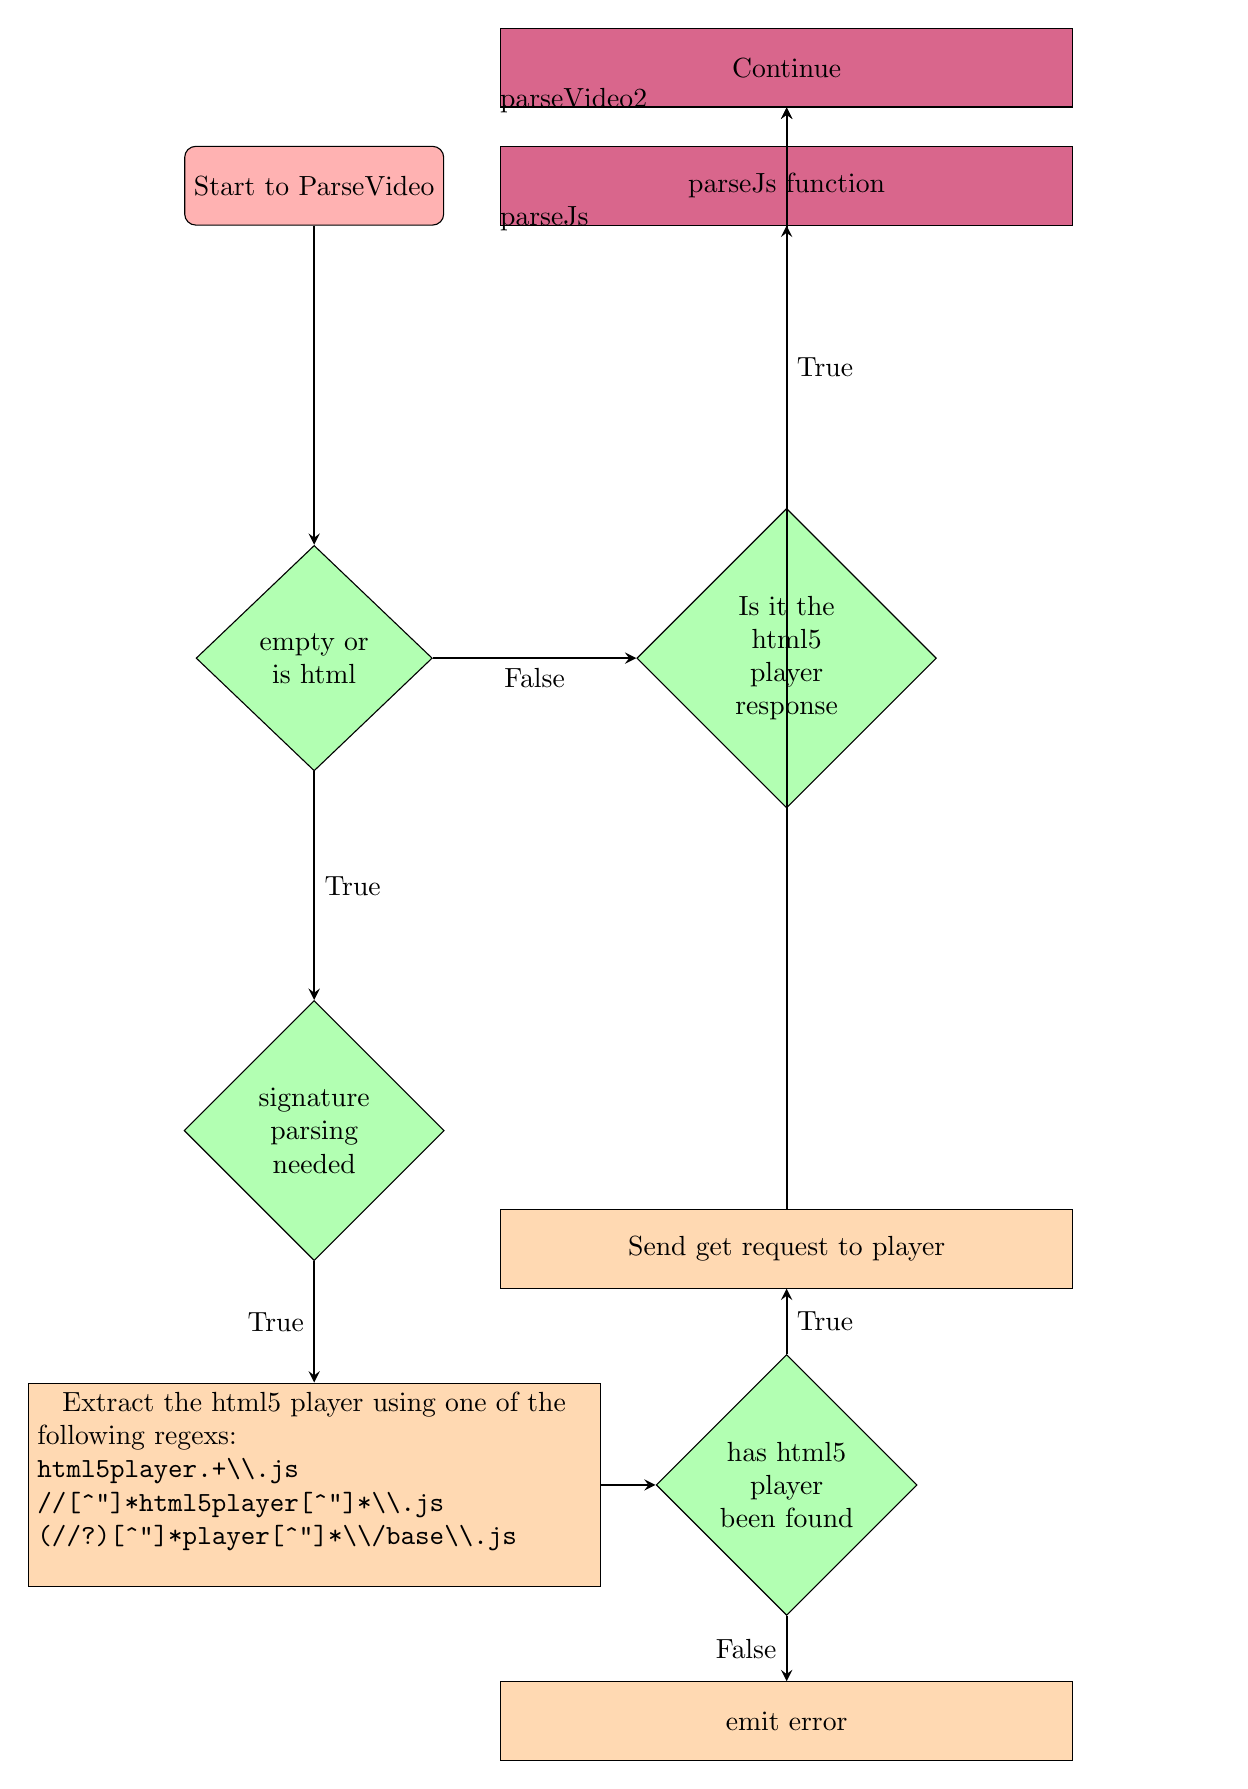
\begin{tikzpicture}[node distance=6cm]
        \node (start) [startstop] {Start to ParseVideo};
        
        %This is for ifHtml if statement
        \node (ifHtml) [decision, below of=start] {empty or is html};
        \node (ifSigparse) [decision, below of=ifHtml] {signature parsing needed};
        \node (ifJs) [decision, right of=ifHtml] {Is it the html5 player response};

        \draw [arrow] (start) -- node {} (ifHtml);
        \draw [arrow] (ifHtml) -- node[anchor=west] {True} (ifSigparse);
        \draw [arrow] (ifHtml) -- node[anchor=north] {False} (ifJs);

        \node (getHtmlPlayer) [process, yshift=1.5cm, below of=ifSigparse] {
                Extract the html5 player using one of the following regexs:\newline
                \verb!html5player.+\\.js!\newline
                \verb!//[^"]*html5player[^"]*\\.js!\newline
                \verb!(//?)[^"]*player[^"]*\\/base\\.js!\newline
        };
        \draw [arrow] (ifSigparse) -- node[anchor=east] {True} (getHtmlPlayer);

        %This is the ifHtmlPlayer if statement
        \node (ifHtmlPlayer) [decision, right of=getHtmlPlayer] {has html5 player been found};
        \node (html5PlayerFalsetFound) [process, yshift=3cm, below of=ifHtmlPlayer] {emit error};
        \node (html5PlayerFound) [process, yshift=-3cm, above of=ifHtmlPlayer] {Send get request to player};

        \draw [arrow] (getHtmlPlayer) -- node {} (ifHtmlPlayer);
        \draw [arrow] (ifHtmlPlayer) -- node[anchor=west] {True} (html5PlayerFound);
        \draw [arrow] (ifHtmlPlayer) -- node[anchor=east] {False} (html5PlayerFalsetFound);

        %js player if statement
        \node (parseJs) [process, hyperlink node=parseJs, fill=purple!60, above of=ifJs] {parseJs function};
        \draw [arrow] (ifJs) -- node[anchor=west] {True} (parseJs);

        \node (continue) [process, yshift=-4.5cm, hyperlink node=parseVideo2, fill=purple!60, above of=parseJs] {Continue};

        \draw [arrow] (parseJs) -- node {} (continue);
        \draw [arrow] (html5PlayerFound) -- node {} (continue);
    \end{tikzpicture}
\end{figure}

\begin{figure}
    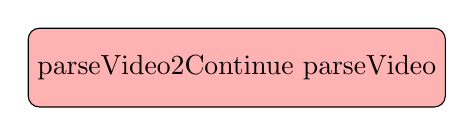
\begin{tikzpicture}[node distance=6cm]

        \node (start) [startstop] {\hypertarget{parseVideo2}{Continue parseVideo}};

    \end{tikzpicture}
\end{figure}

\begin{figure}
    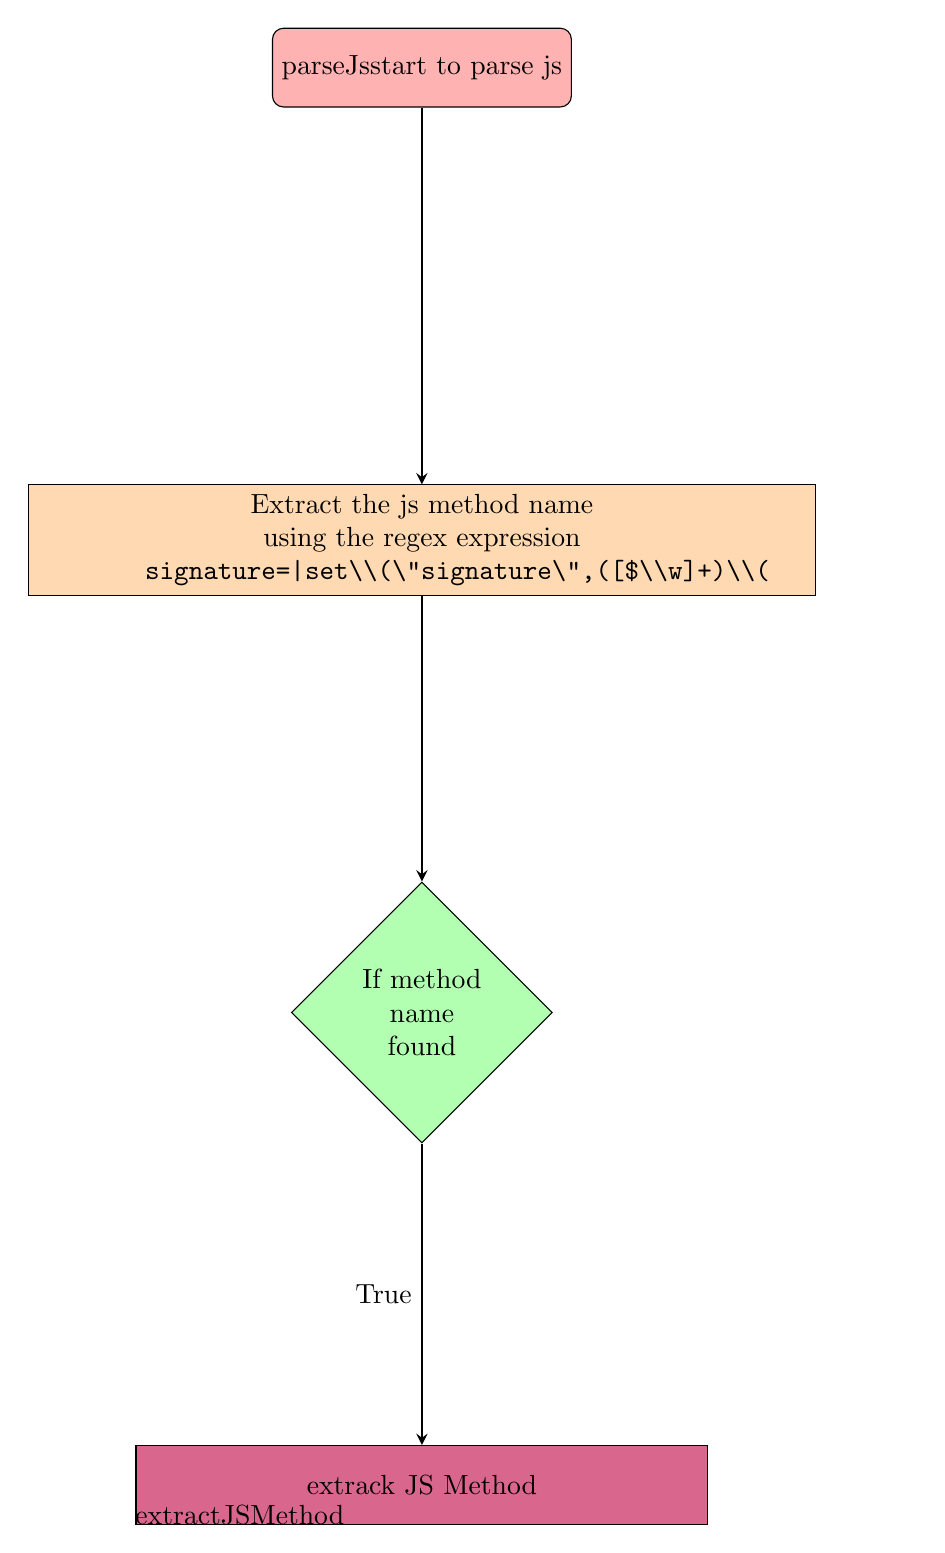
\begin{tikzpicture}[node distance=6cm]

        \node (start) [startstop] {\hypertarget{parseJs}{start to parse js}};
        \node (regexExpression) [process, below of=start, minimum width=10cm] {
                Extract the js method name using the regex expression
                \verb!signature=|set\\(\"signature\",([$\\w]+)\\(!
            };

        \node (ifFound) [decision, below of=regexExpression] {If method name found};
        \node (methodCall) [process, fill=purple!60, hyperlink node=extractJSMethod, below of=ifFound] {extrack JS Method};

        \draw [arrow] (start) -- node {} (regexExpression);
        \draw [arrow] (regexExpression) -- node {} (ifFound);
        \draw [arrow] (ifFound) -- node[anchor=east] {True} (methodCall);

    \end{tikzpicture}
\end{figure}

\begin{figure}
    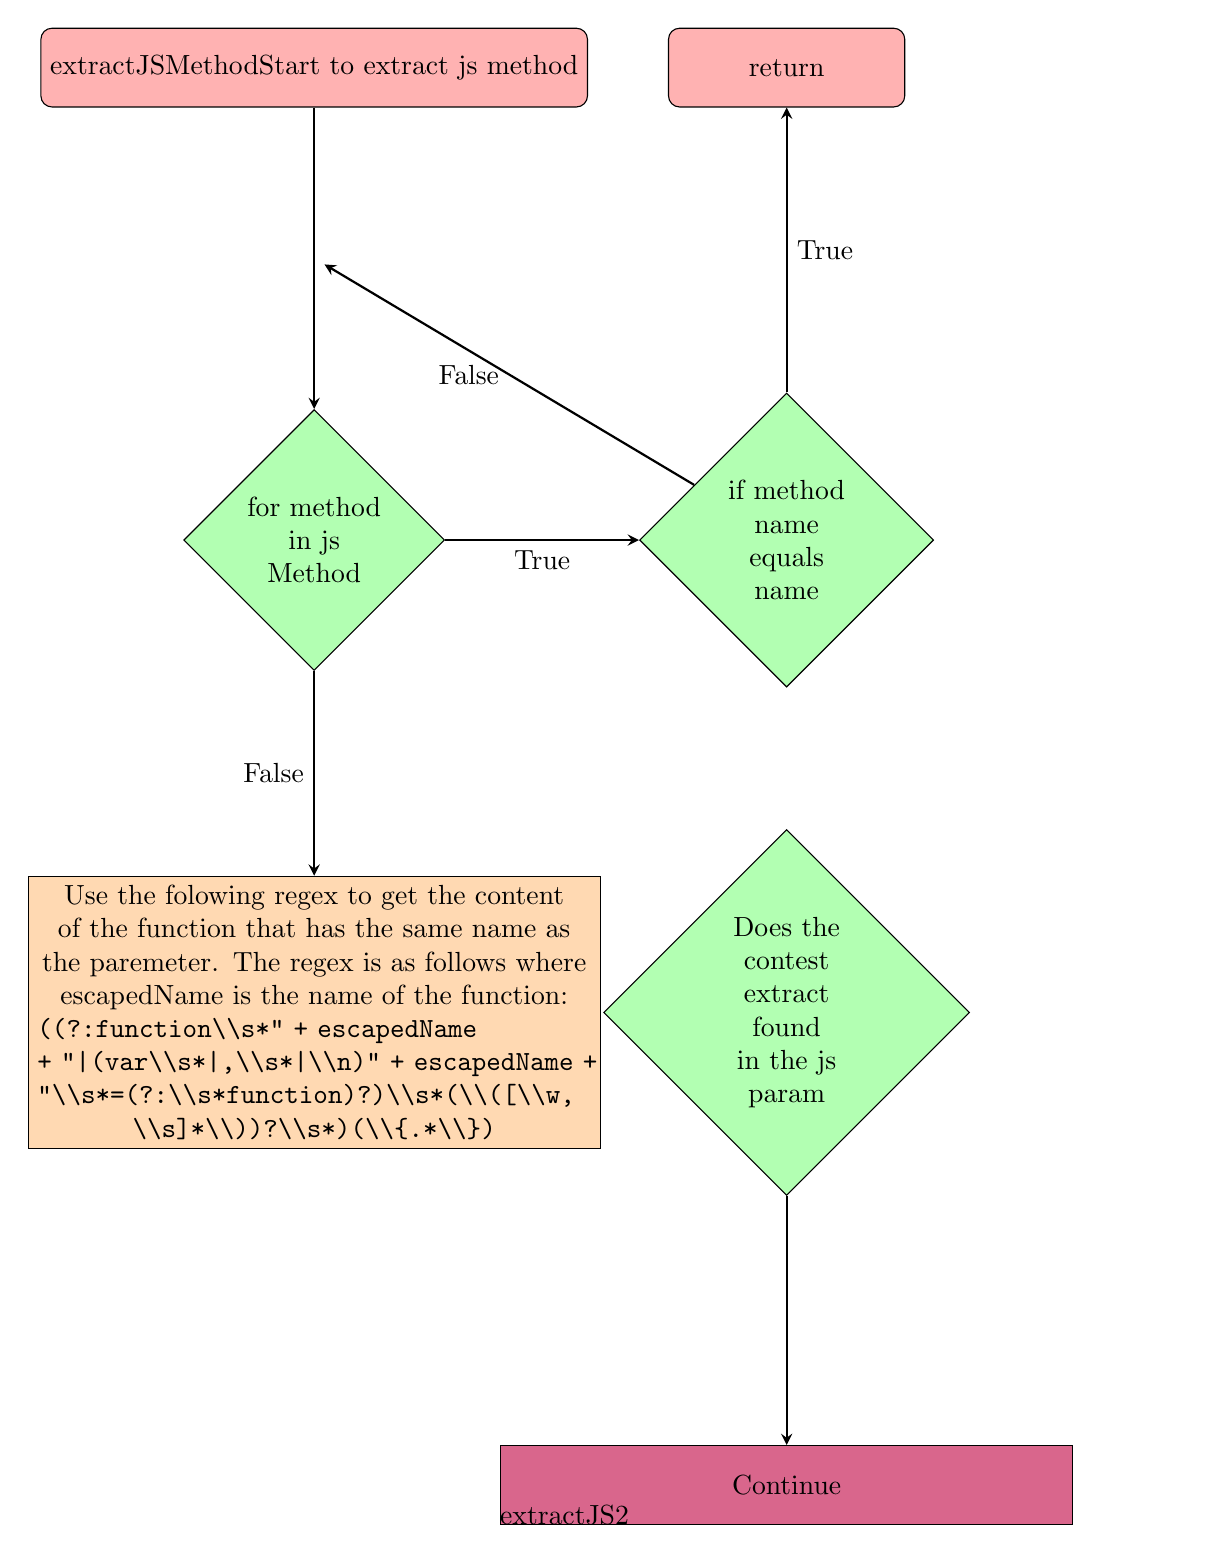
\begin{tikzpicture}[node distance=6cm]

        \node (start) [startstop] {\hypertarget{extractJSMethod}{Start to extract js method}};
        \node (checkIfCompleted) [decision, below of=start] {for method in js Method};
        \node (ifComplete) [decision, right of=checkIfCompleted] {if method name equals name};
        \node (isCompleted) [startstop, above of=ifComplete] {return};


        \draw [arrow] (start) -- node (CheckCompleteforarrow) {} (checkIfCompleted);
        \draw [arrow] (checkIfCompleted) -- node[anchor=north] {True} (ifComplete);
        \draw [arrow] (ifComplete) -- node[anchor=west] {True} (isCompleted);
        \draw [arrow] (ifComplete) -- node[anchor=east] {False} (CheckCompleteforarrow);
        
        \node (firstFunctionRegex) [process, below of=checkIfCompleted] {Use the folowing regex to get the content
        of the function that has the same name as the paremeter. The regex is as follows where escapedName is the
        name of the function:

        \verb!((?:function\\s*" + escapedName!\newline
        \verb!+ "|(var\\s*|,\\s*|\\n)" + escapedName +!\newline
        \verb!"\\s*=(?:\\s*function)?)\\s*(\\([\\w,!\newline
        \verb!\\s]*\\))?\\s*)(\\{.*\\})!};

        \draw [arrow] (checkIfCompleted) -- node[anchor=east] {False} (firstFunctionRegex);

        \node (checkIfContentMatchParam) [decision, right of=firstFunctionRegex] {Does the contest extract found in the js param};
        \node (extractJsContinued) [process, hyperlink node=extractJS2, fill=purple!60, below of=checkIfContentMatchParam] {Continue};
       \draw [arrow] (checkIfContentMatchParam) -- node {} (extractJsContinued); 

    \end{tikzpicture}
\end{figure}

\begin{figure}
    \begin{tikzpicture}[node distance=6cm]
        \node (start) [startstop] {\hypertarget{extractJS2}{extractJS method part 2}};
        \node (createObject) [process, below of=start] {Initializes a object of type jsMethod (Fig ~\ref{fig:Struct layout})};
        \node (setProperties) [process, below of=createObject] {Set the name, code properties of jsMethod and add to jsMethods
                                                                property};
        \node (ifMethodCodeNotEmpty) [decision, right of=setProperties] {Is the object code empty};
        \node (regex) [process, above of=ifMethodCodeNotEmpty, yshift=-1.5cm] {Use the follow regex: 
            \verb!([\\w\\$]+)(?:[\\w\\.\\$])*\\s*!\newline
            \verb!(\\([\\w\\s,\"\\$]*)\\)!};
        \node (recursive) [process, above of=regex, yshift=-1.5cm] {The regex should find functions called inside. After finding these functions
        call \hypertarget{extractJSMethod}{extractJS} with the name and code as arguments};

        \node (stop) [startstop, above of=recursive] {Finish};

        \draw [arrow] (start) -- node {} (createObject);
        \draw [arrow] (createObject) -- node {} (setProperties);
        \draw [arrow] (setProperties) -- node {} (ifMethodCodeNotEmpty);
        \draw [arrow] (ifMethodCodeNotEmpty) -- node[anchor=east] {False} (regex);
        \draw [arrow] (regex) -- node {} (recursive);
        \draw [arrow] (recursive) -- node {} (stop);


        \node (escapeRegex) [process, below of=checkIfCompleted] {Find the contents of the
            method from the name using a regular expression};
        \node (ifFunctionContentFound) [decision, below of=escapeRegex] {Has the content of
            the function been found};
        \node (FunctionContentHasBeenFound) [process, below of=ifFunctionContentFound] {
            Create a jsMethod struct (Fig ~\ref{fig:Struct layout} ) and set the code
            and name properties to that found by the regex};

    \end{tikzpicture}
\end{figure}
\subsection{DataTable}\label{DataTable}

\begin{center}
    \begin{tabular} { | c | c | c |}
        \hline
        Variable Name     &     Type     &               Summary                          \\ \hline
        \multicolumn{3} {| c |}{Main function in Window.cpp}                              \\ \hline
        app               &  QApplication& This is part of the Qt api and is              \\ 
                                         &&used to initialize the necessary               \\ 
                                         &&things                                         \\ \hline
        mainWidget        &  Object of   & This is the only object of the                 \\
                          &  MainWidget  &MainWidget class which is descirbed             \\
                                         &&here at Fig ~\ref{fig:MainWidget}              \\ \hline
        downloadWidget    &  Object of   & This is the only object of the                 \\
                          &  DownloadTab &DownloadWidget class that is one of             \\
                                         &&the main tab classes. It's                     \\
                                         &&functionality is described here at             \\
                                         &&Fig ~\ref{fig:DownloadTab Diagram}             \\ \hline
        libraryTab        &  Object of   & This is the only object of the                 \\
                          &  LibraryTab  &libraryTab class. It is described               \\
                                         &&here in Fig ~\ref{fig:LibraryTab class layout} \\ \hline
        window            &  Object of   & This is the only object of the class.          \\
                          &  MainWindow  & It is described here ~\ref{fig:MainWindow}     \\ \hline

                         
    \end{tabular}
\end{center}

\end{document}
